\bartchapterimage{rampressure}
\bartthumb{thumb_rampressure}
\chapter{Luminosity function}
%
\section{Determine the LF}
%
\postit{There is very lot of words in this note but I can't stop to write, else
the world will end!}{5}

When we want to compare the results from our galaxy group finder to other
existing algorithms, we have to compare a flux limited catalogue with our
algorithm. But as said before, our algorithm works on a double complete sample
of galaxies. So, we need to develop a flux limited version of our algorithm.

The problem when working with a flux limited sample of galaxies is that we must
correct for missing galaxies. The galaxies observed by the survey can be seen
just when they are brighter than a luminosity limit which depends on the
redshift (the distance of the galaxy). We can determine this luminosity easily
by the theory:
%
\begin{equation}
    L_{\lim}\pg{z}\pd={{\pg\frac{d_{\rm{lum}}\pg{z}\pd}{10pc}\pd}^2}10^{0.4\pg{M_{\odot}-m_{\lim}}\pd}
\end{equation}
%
with $m_{\mathrm{\lim}}$ the magnitude limit of the survey and $M_{\odot}$ the
absolute magnitude of the sun, all in the same band filter. This luminosity is
in unit of sun luminosity. In ours groups, when they are at a distance above
the distance limit to see galaxies with the luminosity threshold of the
catalogue, some galaxies are missing because they can't be seen. In order to
correct for the number of missing galaxies, we have to know the distribution of
galaxy luminosities. With this luminosity function (LF), we can calculate the
``fraction'' of galaxy luminosities in mean that we can see:
%
\begin{equation}\label{eq:correc}
    f\pg{L_{\lim}{\pg{z}\pd}}\pd=\frac{\int_{L_{\lim}\pg{z}\pd}^{\infty}L\phi{\pg{L}\pd}\dd{L}}{\int_{L_{thres}}^{\infty}L\phi{\pg{L}\pd}\dd{L}}
\end{equation}
%
where $\phi\pg{L}\pd$ is the LF\@. So determining this LF is useful to correct
for missing galaxies.

But, as we expect with the goal of this thesis, it's clear for us that
properties of galaxies depend on the environment. So the luminosity function
may probably depend on the host halo. The LF have to depend on different
characteristics of the halo. The unique ``observable'' property is the virial
mass so we want that the LF depends on it. This is the better way to correct
for the incompleteness of groups, with a particular correction for each group.
\com{Put something in order to justify physically this dependence on the halo
mass!} Resulting from this idea, the LF used in (\ref{eq:correc}) becomes a
conditional LF, which is the LF in groups of a given halo mass:
%
\begin{equation}
    \phi\pg{L}\pd\rightarrow\phi\pg{L|M}\pd%
\end{equation}
%
\postit{There is very lot of words in this note but I can't stop to write, else
the world will end!}{5}

In galaxy groups, we separate galaxies in two classes: centrals and satellites.
Centrals are expected to be the most massives galaxies in groups, and
consequently, it's probable that the central is the brighter galaxy. A
consequence is that if we can't see the central galaxy, we can't see other
galaxies in the group and the correction is not needed because we don't know
how to correct for incompleteness. So for the correction we just need to
constrain the distribution of luminosities in satellite galaxies.

In practice, we have to choose a functional for this conditional luminosity
function (CLF) which can be easily fitted and integrated to determine the
correction factor in our group luminosities. In studies of the galaxy sample
from the SDSS survey as in \citet{Blanton+05}, the LF has been well fitted by a
double Schechter functional form which can be written:
%
\begin{equation}\label{eq:dblsch}
    \phi\pg{L}\pd=\pg{\phi_1^*{\pg{\cfrac{L}{L_*}}\pd}^{\alpha_1}+\phi_2^*{\pg{\cfrac{L}{L_*}}\pd}^{\alpha_2}}\pd\exp\pg{-\pg{\cfrac{L}{L_*}}\pd}\pd%
\end{equation}

Now we assume that the CLF have the same form that (\ref{eq:dblsch}). The
dependence on the halo mass $M$ is taken with the parameters of the double
Schechter (DS). For example $\alpha_1\rightarrow\alpha_1\pg{M|\theta}\pd$,
where the functional form of this dependence is not given explicitly here, and
$\theta$ is a set of parameters relative to the function used to describe the
dependence with halo mass. The number of parameters in $\theta$ can vary
greatly, depending on the function used.

The form of this dependence can't be determine in advance when we want to fit
the CLF on the data. For example in the SDSS, we have to know in advance the
properties of the groups in order to choose a certain dependence for the
parameters of the DS with the virial mass. So, for testing the viability of
this method, we have to select a functional that describes correctly the
modulation of the parameters with the halo, and samples of galaxies that can
give us this information are present in outputs of semi-analytical models
(SAM). In such samples, we know in which group a galaxy is, and the virial mass
of the host halo is known too. To validate this method of correction for
incompleteness, we can test it in mock galaxy catalogues.
%
\subsection{Estimating parameters}
%
We need to use a method for estimating the parameters that fit well the data
(real or simulated). When working with distribution function, it is common and
better to use the maximum likelihood estimation defined as:
%
\begin{equation}\label{eq:like}
    \mathcal{L}\pg{\theta|X}\pd=\prod_i{p_i\pg{X_i|\theta}\pd}
\end{equation}
%
where $X$ is the set of data (in our case the luminosity $L$) and $\theta$ the
set of parameters of the model that have to be estimated.

If we consider Bayesian statistics, the likelihood is defined as
$p\pg{X|\theta}\pd$ and it seems to be incoherent. But using the Bayes's
theorem, we can see that \emph{our} likelihood is in reality the posterior
distribution which is proportional to the likelihood in the definition of
Bayesian statistics, multiply by a prior. But we don't have any prior on the
parameters distribution (which can be discussed\ldots). So, if we take a
constant for the prior (probability equal for each parameter), we get same
results.

It's more convenient to use the logarithm of the likelihood in order to prevent
numerical problems when calculating the likelihood. The product in
(\ref{eq:like}) becomes at this moment a sum, and the computation is
simplified. It's easier too to minimize a function numerically so we rewrite
it.
%
\begin{equation}\label{eq:loglike}
    -\log\mathcal{L}\pg{\theta|X}\pd=-\sum_i{\log\pg{p_i\pg{X_i|\theta}\pd}\pd}
\end{equation}

We define $p_i\pg{X_i|\theta}\pd$ as the probability to get the value $X_i$
given the parameters $\theta$, so it's the probability density. To determine
this density, we need to calculate the number of ``points'' in the sample which
are between $X_i$ and $X_i+\dd{X_i}$ compare to the total number of points in
the set $X$:
%
\begin{equation}
    p_i\pg{X_i|\theta}\pd\dd{X_i} = \cfrac{\dd{N_i}}{N_{\mathrm{tot}}}
\end{equation}

By definition of the CLF, which is the number of galaxies by unit of volume
comprised between $L$ and $L+\dd{L}$ at a given halo mass $M$, we can write:
%
\begin{equation}
    \dd^2{N}=\phi\pg{L|M}\pd\dd{L}\dd{V}
\end{equation}
%
Summing on all the volume in which we are working, we get:
%
\begin{equation}
    \dd{N}=\phi\pg{L|M}\pd\dd{L}
\end{equation}
%
\com{Because we are working in limited volume region, we can rewrite the
    probability density as:
%
\begin{equation}
    p_i\pg{L_i|\theta}\pd\dd{L_i}\dd{V} = \cfrac{\dd^2{N_i}}{N_{\mathrm{tot}}}
\end{equation}}
%
So we can write:
%
\begin{equation}
    p_i\pg{L_i|\theta}\pd\dd{L_i} = \cfrac{\phi\pg{L_i|M}\pd\dd{L_i}}{N_{\mathrm{tot}}}
\end{equation}
%
and the total number of galaxies is just:
%
\begin{equation}
    N_{\mathrm{tot}}=\int_{L_{\mathrm{thres}}}^\infty{\phi\pg{L|M}\pd\dd{L}}
\end{equation}
%
In this way, the density probability for the DS can be written:
%
\begin{equation}
    p_i\pg{L_i\left|\alpha_1, \alpha_2, M_*, \cfrac{\phi_2^*}{\phi_1^*}\right.}\pd=\cfrac{\pg{{\pg{\cfrac{L}{L_*}}\pd}^{\alpha_1}
    +\cfrac{\phi_2^*}{\phi_1^*} {\pg{\cfrac{L}{L_*}}\pd}^{\alpha_2}}\pd\exp\pg{-\pg{\cfrac{L}{L_*}}\pd}\pd}{\pg{\Gamma\pg{1+\alpha_1,
    \cfrac{L_{\mathrm{thres}}}{L_*}}\pd+\cfrac{\phi_2^*}{\phi_1^*}\Gamma\pg{1+\alpha_2,\cfrac{L_{\mathrm{thres}}}{L_*}}\pd}\pd}
\end{equation}
%
where $\Gamma\pg{a,x}\pd=\int_x^{\infty}e^{-t}{t^{a-1}}\dd{t}$ is the
incomplete gamma function.

The principle of the estimation by the method of the maximum likelihood is that
when we maximize the likelihood relatively to the parameters $\theta$, we get
the maximum of probability, likelihood, of having the parameters that
correspond denoted $\hat{\theta}$. The parameters $\hat{\theta}$ are the
parameters that best fit the data according to the functional form assumed for
the CLF.\@ Numerically we minimize the equation (\ref{eq:loglike}).

There are many ways of doing such a minimization. When the probability density
isn't too complex, $\hat{\theta}$ can be determined analytically. But in this
case, with the DS, the incomplete gamma function prevent us to do it in this
way. So we are constrained to use numerical methods in order to minimize the
likelihood. Many algorithms exist to do this job like Powell's method,
Newton-Raphson's method, etc\ldots, but they share the same problem: when they
find a minimum, we can't know if it is the global minimum or if it is a local
minimum. The result depends on the initial starting point of the algorithm in
the parameter space. Some other methods try, using Monte-Carlo methods, to do a
better exploration of this parameter space, allowing some ``jumps'' to other
regions in order to see if there isn't a best minimum near. An example of such
an algorithm is the simulated annealing method which implement the cooling of a
material where the function to minimize becomes the energy of the system and a
fictive temperature $T$ is introduce to allow some temperature jumps. But it is
not always sure that we get the global minimum. Moreover, we can't easily
determine errors on the estimation of the parameters, except using bootstraps
or jackknife techniques which need many estimation of the parameters varying
the sample which may be expensive in calculation time.

We have chosen to use the Markov Chains Monte Carlo method (MCMC) to minimize
our function. This method is the better in all the universe. \com{Explain
why!}. We can estimate easily with results of the algorithm the errors on the
parameters.

We will now resume the result of works on mock catalogues of our method of
estimating the CLF\@.
%
\subsection{Tests on mock catalogues}
%
There is two steps in order to determine the dependence on the halo mass of the
parameters of the DS model. First, we have to determine what is the best
functional form to fit this dependence which can be done on a complete sample
of galaxy. Secondly, see if we can recover this parametrisation and modulation
with a flux limited sample of this galaxies to know if the method works well
when applied in a real survey.
%
\subsubsection{Complete sample}
%
In order to determine the dependence on the halo mass of the parameters, we use
a complete sample of galaxies taken from the outputs of the SAM of
\citet{Guo+11} applied on dark matter halos from the Millennium II run. We
limit our sample of galaxies from this catalogue to galaxies with a luminosity
such that the absolute magnitude in the $r$ band is $M_r<-12$. For each galaxy,
we have the virial mass of the halo which contains this galaxy. Our complete
sample is defined just as this galaxy catalogues from \citet{Guo+11} with the
truncation on the data through the $r$ band magnitude.

First, we determine what is the best model for the ``total'' CLF, \textit{i.e.}
the LF when we don't do a segregation with the halo mass. We have tried to
adjust a simple Schechter and a double Schechter. Results are shown on figure
(\ref{fig:fitguo}).
%
\begin{figure}[ht]
    \centering
    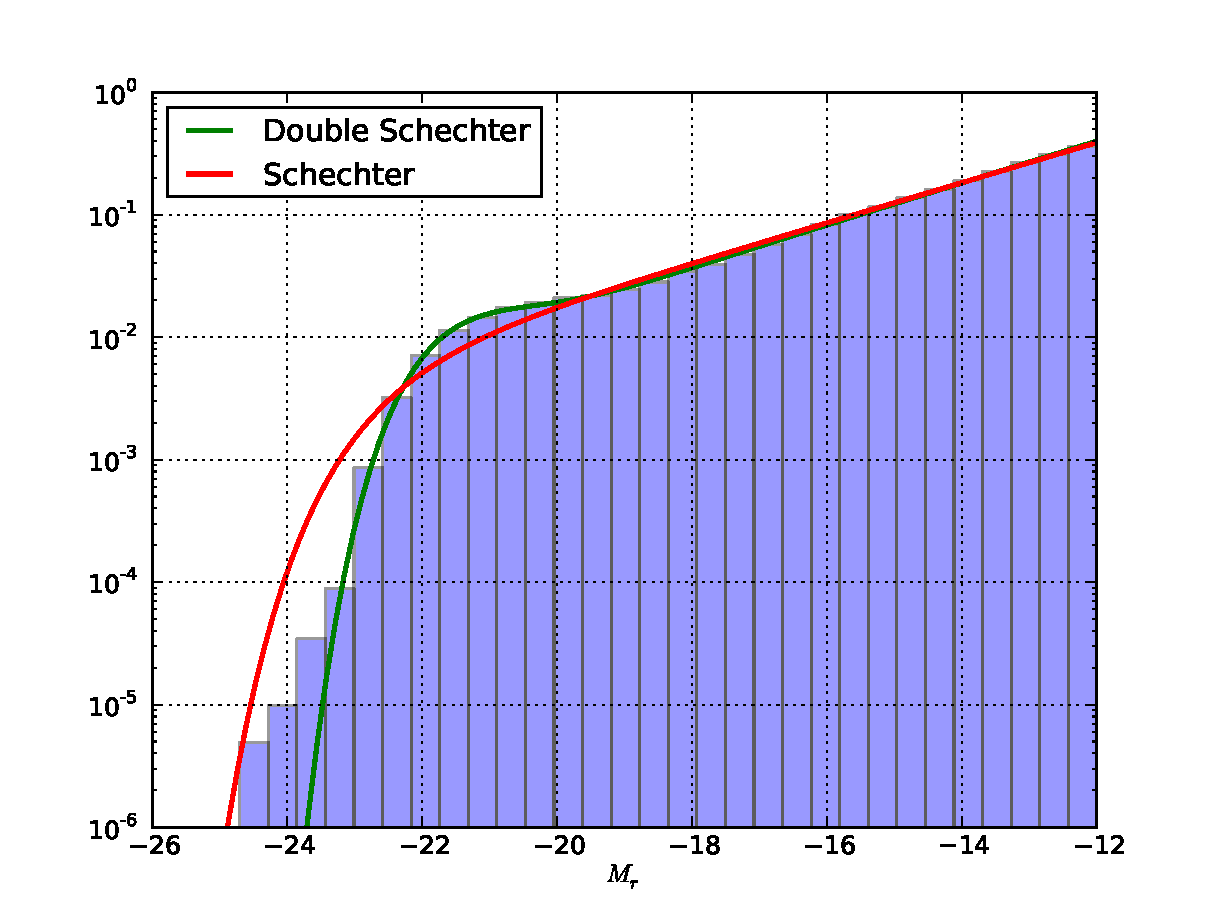
\includegraphics[width=0.5\linewidth]{MCMCfitGUO}
    \caption{Results of the fit on the data in blue with a Schechter
        distribution in red and a double Schechter distribution in green. The
        double Schechter fit is better because this form allow to constrain the
        two galaxy populations we can see in our sample: a low population with
    high slope and a brighter population with a more little slope in absolute
value.}
\label{fig:fitguo}
\end{figure}
%
We can see that the minimization works well because the fit seems to be good
enough in the figure. The double Schechter fits better the data than the simple
Schechter because we can constrain with this form the two populations of
galaxies in the sample from the \citet{Guo+11} SAM\@. We see that there is a
low population with high slope and a brighter population with a slope more
little. Differences with the data at luminous galaxies is due to the fact that
the number of galaxies with $M_r<-24$ is very low, in some bins there is just
one galaxy. But we need a quantitative proof of this fit. We use for that the
Kolmogorov-Smirnov test ans the P-Value associated.\com{TODO\@: KS test on the
fit in order to get a good idea of the robustness of the fit.}
\begin{figure}[H]
    \centering
    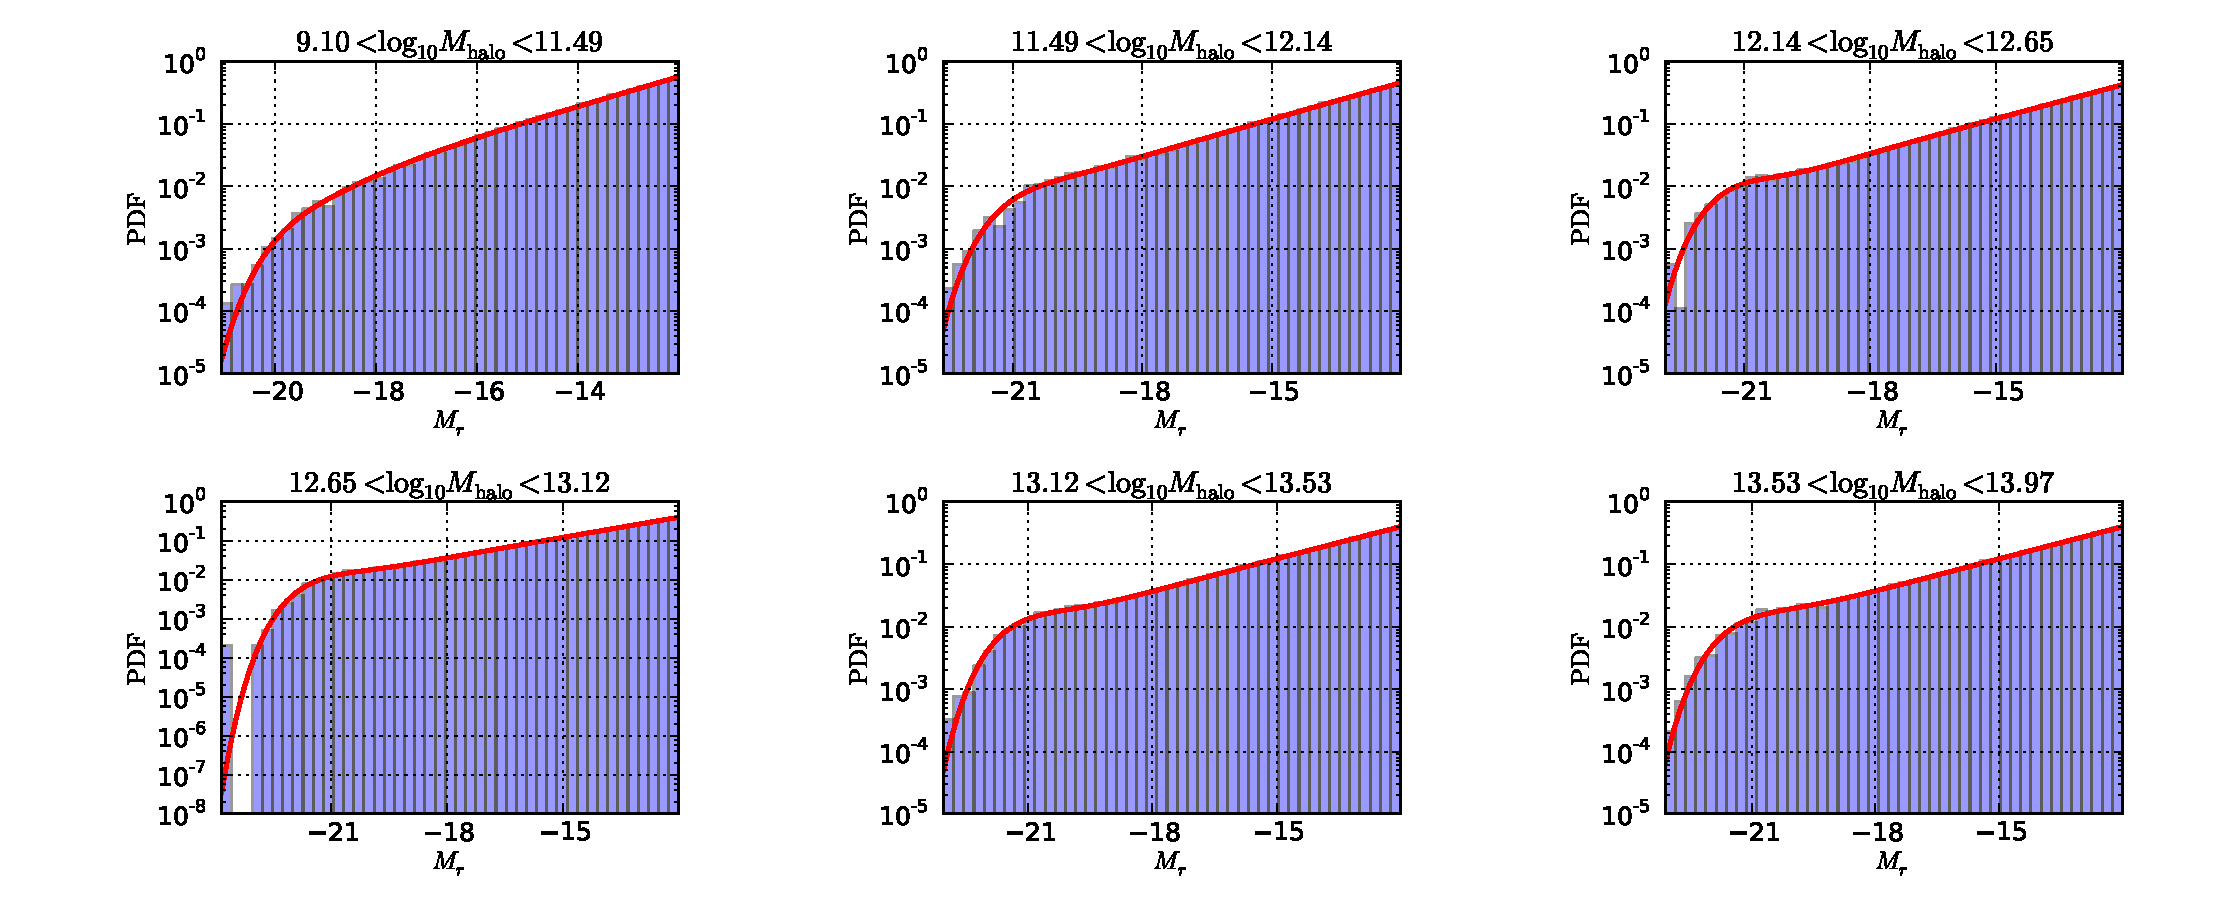
\includegraphics[width=\linewidth]{FitDblSchechterGuo}
    \caption{Results of the fit for the double Schechter distribution in
    different bins of halo mass. In blue the PDF of the data, and in red the
fit with parameters obtained from the MCMC algorithm.}
\label{fig:fitguodblsch}
\end{figure}

Happy to see that the minimization is good, we want to see the modulation of
the parameters of the DS with the halo mass. For doing that we take galaxies in
bins of the certain width in halo mass, and we compute the parameters that fit
well the data in each, as previously. This modulation is represented in the
figure (\ref{fig:modsch}).
%
\begin{figure*}[p]
    \centering
    \begin{minipage}{\linewidth}
    \centering
    \subfloat[For a Schechter distribution]{%
        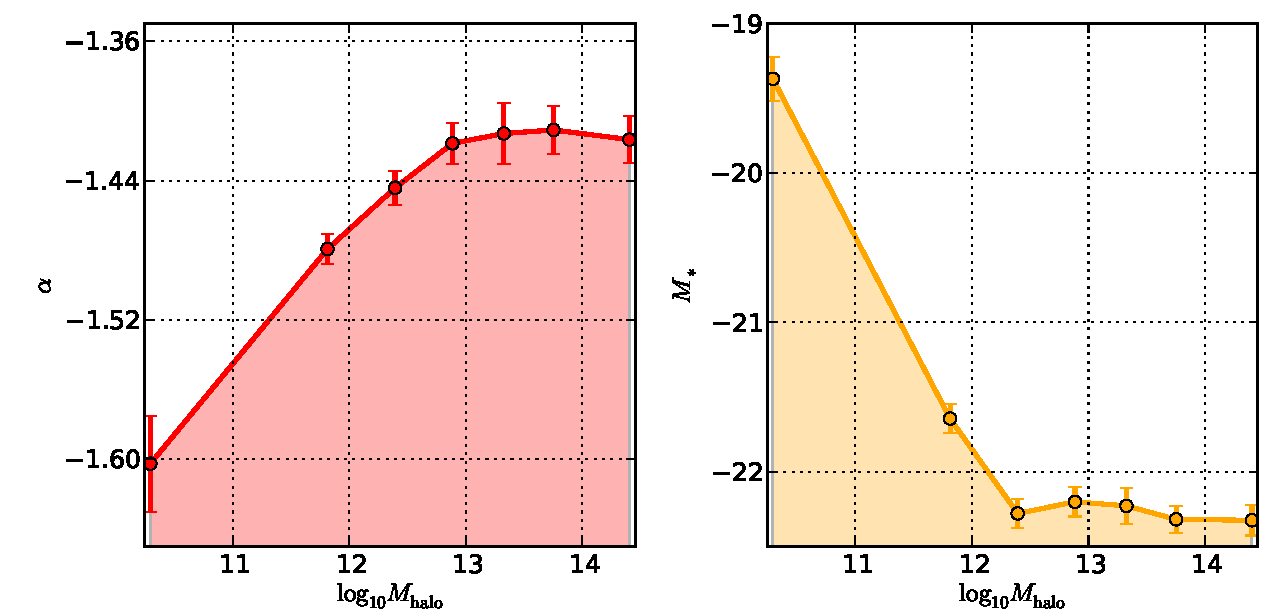
\includegraphics[width=\linewidth]{evolSchechterGuo}
    }
    \end{minipage}
    \begin{minipage}{\linewidth}
    \centering
    \subfloat[For a double Schechter distribution]{%
        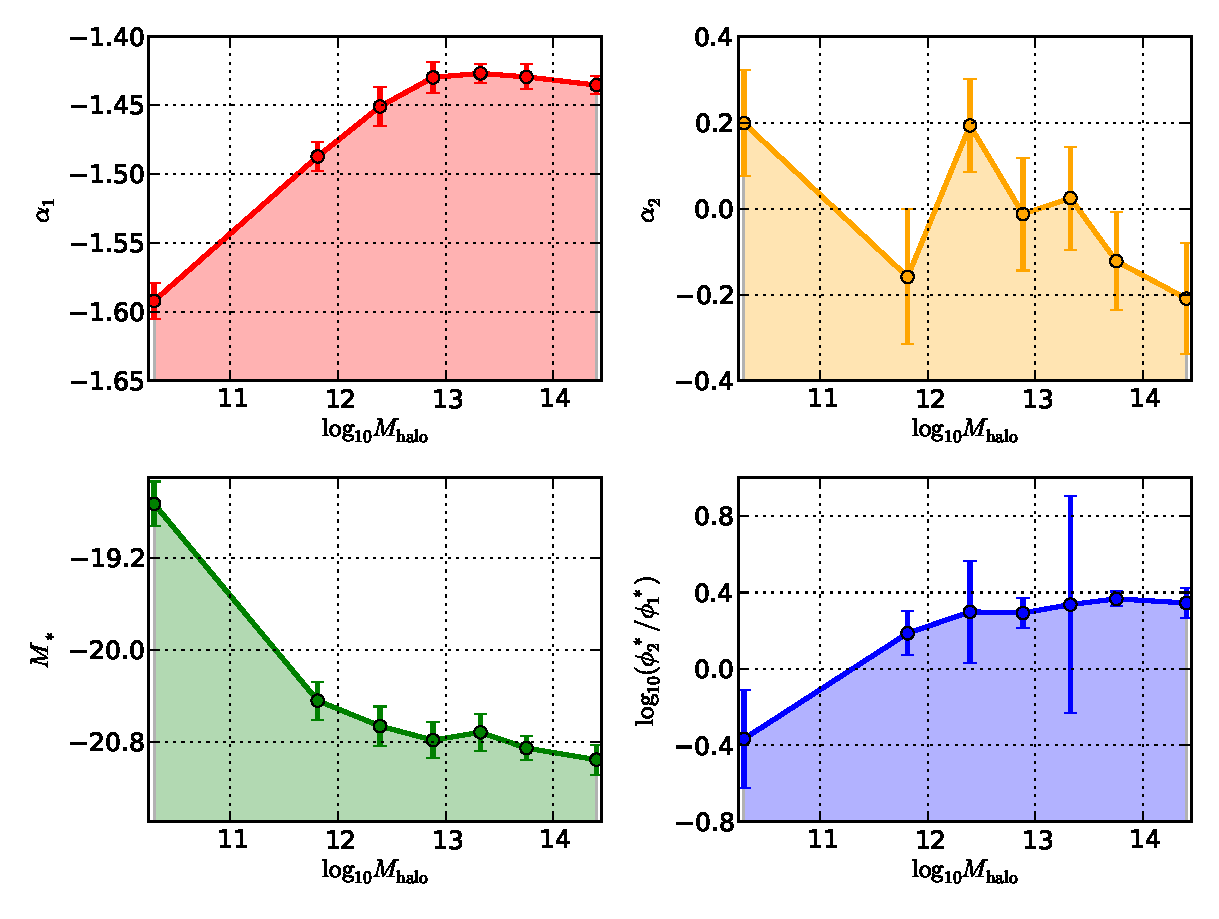
\includegraphics[width=\linewidth]{evolDblSchechterGuo}
    }
    \end{minipage}
    \caption{Modulation of the parameters of both Schechter and
    double Schechter luminosity distributions with the halo mass.}
\label{fig:modsch}
\end{figure*}
%
The resulting fit of the probability density function is shown for the double
Schechter in the figure (\ref{fig:fitguodblsch}).

As we expect, we can see some physics process putted in the SAM in this
figure.\com{To detail.}

Therefore, \com{Verify Cependant$\rightarrow$Therefore.}, we don't see a
particular modulation, \textit{i.e.} a functional form to use for each
parameter of the DS.\@ So we have decided to use polynomials functions to
adjust this modulation. For a given parameter $\theta_i$ we write:
%
\begin{equation}
    \theta_i\pg{M}\pd=\sum_{j=0}^N{a_{ij}{M^j}}
\end{equation}
%
where $N$ is the order of the polynomial.

We now integrate this form of parametrization of the parameters of the DS into
the minimization of the likelihood using directly the halo masses of the
galaxies.

But it doesn't work!!!\com{Some blabla!}
%
\subsubsection{Flux limited sample}
%
Working with a flux limited sample, it's like having gaps into the set of
galaxies. But we know why we are missing this galaxies: we can't see them at a
given distance. Determining the luminosity limit which we can see at redshift
$z$ can be done analytically. So for that we use the STY method.\com{Put Bibtex
of STY and description related to this.} We need to modify the probability
density used in the likelihood to take into account missing data. The procedure
is the following: in order to estimate the likelihood, we have to calculate the
probability density for a galaxy $i$ at the redshift $z_i$ of having a
magnitude between $M_i$ and $M_i+\dd{M_i}$. The probability that a galaxy have
a magnitude $\mathcal{M}$ superior to $M$ is given by:
%
\begin{equation}\label{eq:cumprobfluxlim}
    P\pg\mathcal{M}>M|z\pd=\cfrac{\int_{-\infty}^M{\phi\pg{M'}\pd\rho\pg{z}\pd{f\pg{M'}\pd}\dd{M'}}}
    {\int_{-\infty}^{\infty}{\phi\pg{M'}\pd\rho\pg{z}\pd{f\pg{M'}\pd}\dd{M'}}}
\end{equation}
%
where $f$ is the completeness function and $\rho\pg{z}\pd$ is the redshift
distribution. We can express it like this because the number of galaxies at a
given redshift $z$ with a given magnitude $M$ is $\dd{N}=\phi\pg{M}\pd\dd{M}$
in a given volume. So to avoid the volume dependence, we multiply by the number
of galaxies in a given volume $\rho\pg{z}\pd=\dd{N}/\dd{V}$. So the number of
galaxies with a magnitude between $M$ and $M+\dd{M}$ is
$\dd^2{N}=\phi\pg{M}\pd\rho\pg{z}\pd\dd{M}\dd{V}$. But with the problem of the
completeness, we can see just galaxies with a certain magnitude defined by $f$
so $\dd^2{N}=\phi\pg{M}\pd\rho\pg{z}\pd f\pg{M}\pd\dd{M}\dd{V}$. The
probability (\ref{eq:cumprobfluxlim}) results from this. Calculating the
probability density is straightforward because we have:
%
\begin{equation}
    P\pg\mathcal{M}>M|z\pd=\int_{-\infty}^M{p\pg{M'|z}\pd}\dd{M'}
\end{equation}
%
and so:
%
\begin{equation}
    p\pg{M|z}\pd=\ddp{P\pg\mathcal{M}>M|z\pd}{M}
\end{equation}
%
Finally:
%
\begin{equation}
    p\pg{M_i|z_i}\pd=\dfrac{\phi\pg{M_i}\pd}{\int_{M_{\mathrm{bright}}\pg{z_i}\pd}^{M_{\mathrm{faint}}\pg{z_i}\pd}
    {\phi\pg{M'}\pd\dd{M'}}}
\end{equation}
%
and this defines the new likelihood in the case of a flux limited sample.

We apply this to the incomplete sample generated with the mock algorithm we
have created. Firstly, we have tried to recover the parameters in the mock with
the apparent magnitudes calculated applying a ``K-decorrection''. The results
are very bad. Parameters can't be recovered correctly and with the two models
chosen (simple Schechter and DS). We don't have the same estimations as in the
complete sample, although the flux limited sample is the same as the complete
sample but ``truncated''. It's not clear why this parameters can't be found.
The procedure isn't in cause, but it's possible that the data are the problem.
We think that our method for estimating the K-decorrection have some troubles
when the redshift is higher than 0.2.

For verifying this assumption, we have made more simple flux limited samples.
We know how to generate random variables following a Schechter distribution and
a DS distribution two. We have placed galaxies in a homogeneous universe, up to
few hundred Mpc. We have assigned redshifts to this galaxies according to their
distances $D$ using simply $z=v/c={H_0}{D}/c$. We apply a Schechter
distribution to the galaxies generated, without taking clusters effects into
account. Calculating apparent magnitudes is done subtracting the distance
modulus using galaxies redshifts. We have done the same applying a DS.\@
Results are the followings:
%
\begin{itemize}
    \item We are enable to recover the Schechter parameters used to generate
        the distribution in the flux limited sample. When data are perfect like
        in this situation, there are no troubles.
    \item Using a DS distribution, we have more difficulties in finding those
        parameters used to generate the flux limited sample. The slopes of both
        the low galaxies and brighter galaxies aren't near the true values.
\end{itemize}
%
We think that the number of low galaxies in the flux limited sample isn't not
sufficient to well constrain the slopes in the DS.\@ As a result, the maximum
likelihood can't find real parameters. It's like a degeneracy is present and
the algorithm can't decide to the true parameters.
%
\begin{figure}[htb]
    \centering
    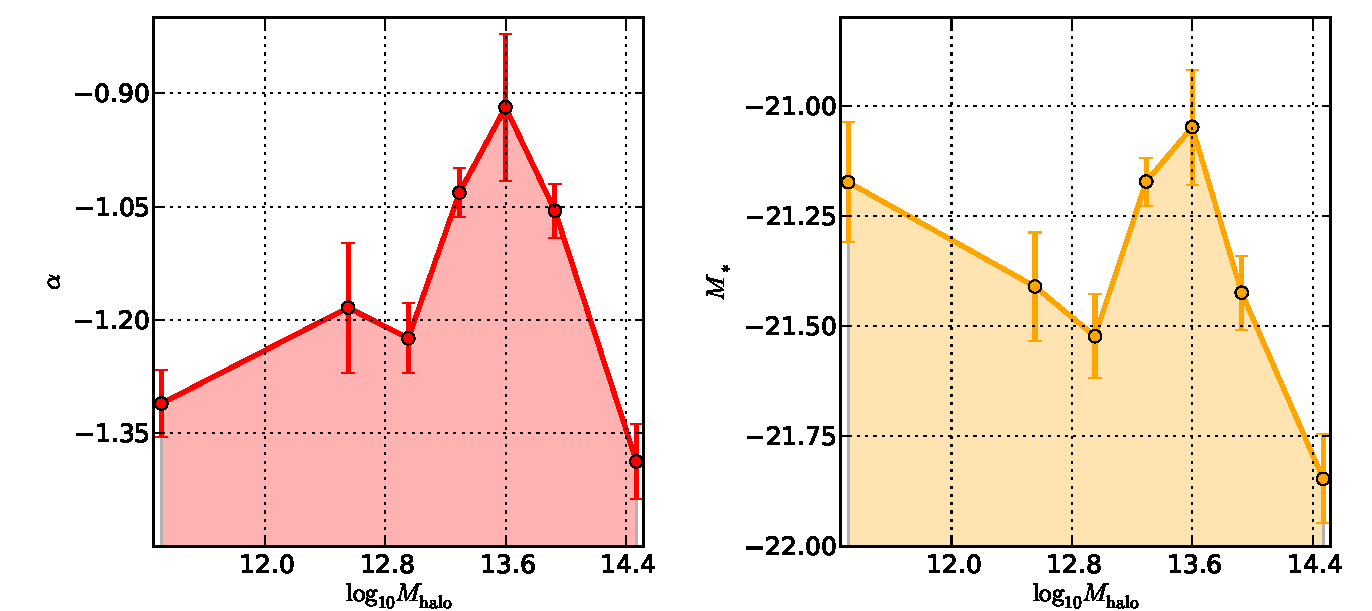
\includegraphics[width=0.8\linewidth]{evolSchechterMock}
    \caption{Modulation of the parameters for a Schechter distribution with the
    halo mass in a mock catalogue constructed with the galaxy catalogue from
the Guo2010a, without taking a K-decorrection for apparent magnitudes of
galaxies.}
\label{fig:parammock}
\end{figure}

So, it's a clue that the K-decorrection isn't good at high redshift and
underestimate the number of galaxies when we apply a flux limit using apparent
magnitudes. We have made an other mock catalogue without this K-decorrection in
order to show that is the real problem. We have extended too the upper
magnitude limit of galaxies in the sample in order to improve the number of low
galaxies to estimate better slopes in the case of the DS\@. The former limit
was -15 in $r$ band magnitude and now we go to -12. So we expect that the
number of low luminosity galaxies increases and improves the parametrization.
All results hereafter and before are for this new limit.

Unfortunately, the increasing number of low mass galaxies and taking no
K-decorrection doesn't improve the estimation of the parameters. Results are
shown in figure (\ref{fig:parammock}).
%
\begin{figure}[htb]
    \centering
    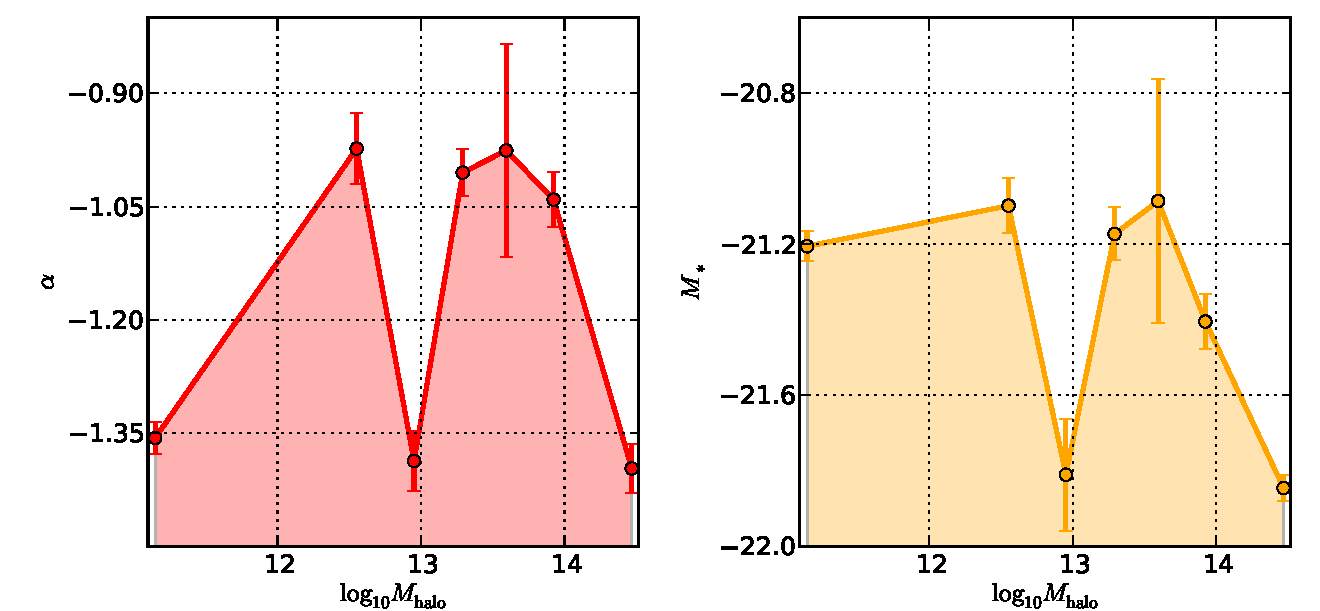
\includegraphics[width=0.8\linewidth]{evolSchechterMockNoBorder}
    \caption{Modulation of the parameters for a Schechter distribution with the
        halo mass in a mock catalogue constructed with the galaxy catalogue
        from the Guo2010a, without taking a K-decorrection for apparent
        magnitudes of galaxies and removing galaxies in groups that are closer
    to the border of cube simulation on the mock's cube.}
\label{fig:parammocknoborder}
\end{figure}

We can see that the modulation of this parameters with the halo mass isn't the
same as in the figure (\ref{fig:modsch}) for the Schechter distribution. It's
not very clear why when we construct the mock catalogue, we can't recover the
same parameters as for the data used to build this mock catalogue. It's maybe a
problem of spatial truncation of data in flux and redshift that may cause some
variations on the intrinsic LF of the data from the galaxy catalogue used for
the mock catalogue. The mock catalogue have a problem: periodic conditions in
the box used in order to build this mock can move away from each other galaxies
belonging to the same group. So in groups of a certain halo mass, we have more
missing data than expected and the estimation of parameters is affected too. To
see if this assumption is correct, we have removed from the sample of galaxies
in the mock catalogue these ones that are in groups too close to the border of
the box in the mock catalogue. The modulation is shown on the figure
(\ref{fig:parammocknoborder}).

We can't find parameters as in the galaxy catalogue from \citet{Guo+11} both
with modulation of the halo mass and for global data. The behaviour is the same
as the latter situation.
%
\begin{figure}[htb]
    \centering
    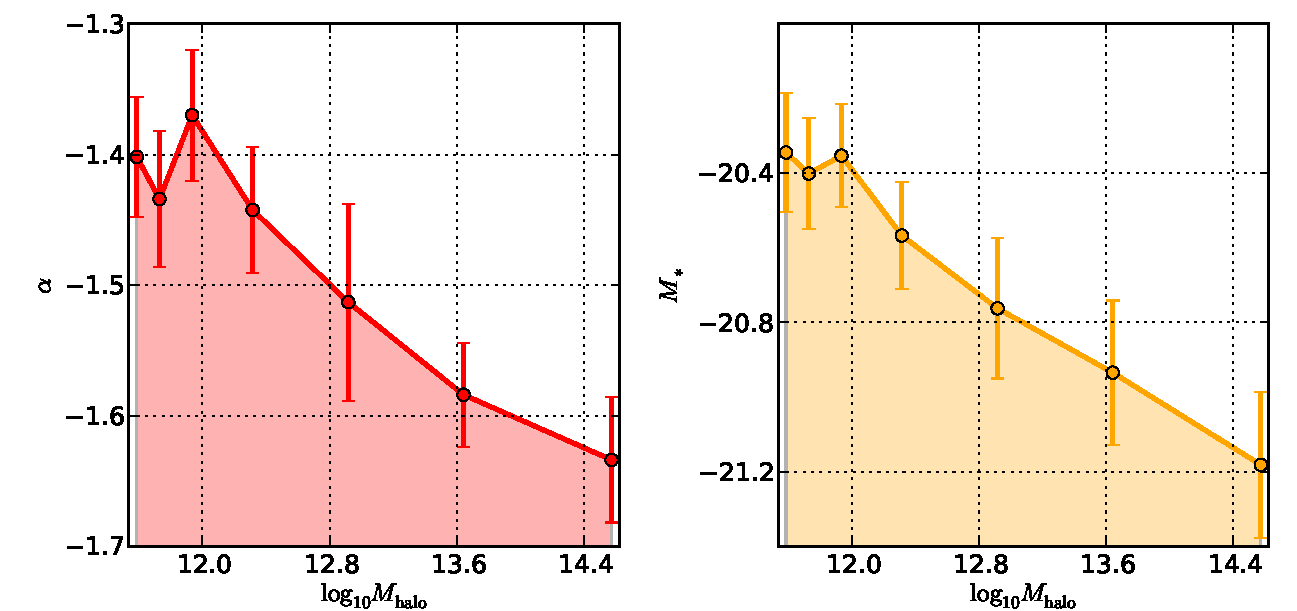
\includegraphics[width=0.8\linewidth]{evolSchechterLinGalPop}
    \caption{Modulation of the parameters for a Schechter distribution with the
        halo mass in the sample of galaxy constructed using a HOD model, and
        imposing a linear evolution of the parameters with halo mass. We have
        imposed that $\alpha$ goes from -1.2 to -1.7 and $M_*$ from -19.5 and
        -21.5 between the extreme halo mass of the
    simulation.}
\label{fig:paramschlin}
\end{figure}

The last test to understand why we can't find the same parameters is described
in what follows. We have used the algorithm described in the appendix \com{add
the description in the appendix to generate a galaxy population from a
simulation} in order to create a sample of galaxy following a NFW profil in
halos, with a velocity dispersion calculated using the \citet{ML05} model for
the anisotropy factor. Galaxy luminosities in the halo are generated in order
to have a linear modulation of the parameters of a Schechter distribution with
the halo mass. We imposed this modulation in the data of the galaxy sample
generated with the HOD model of~\cite{Zehavi+11}. The magnitude sample has
$-23<M_r<-12$. The result of this modulation in the complete sample
is shown in figure (\ref{fig:paramschlin}).

We now construct an other mock catalogue using this galaxy sample in order to
see what happened when we fix the modulation in the parameters with the halo
mass in a flux limited sample. Results are shown on the figure
(\ref{fig:paramschlin})

The mock catalogue we have created goes to a redshift of 0.1 while the
mock with the galaxy sample from \citet{Guo+11} is limited to a redshift of
0.3. The modulation of the parameters we have imposed in the galaxy
sample is well recovered. In the case of $M_*$, the estimation is always good,
same with a DS.\@ But there are more uncertainties in finding the slope of the
LF with both Schechter and DS.\@ Slopes are less constrained by the data when
with have a flux limited sample.
%
\begin{figure}[htb]
    \centering
    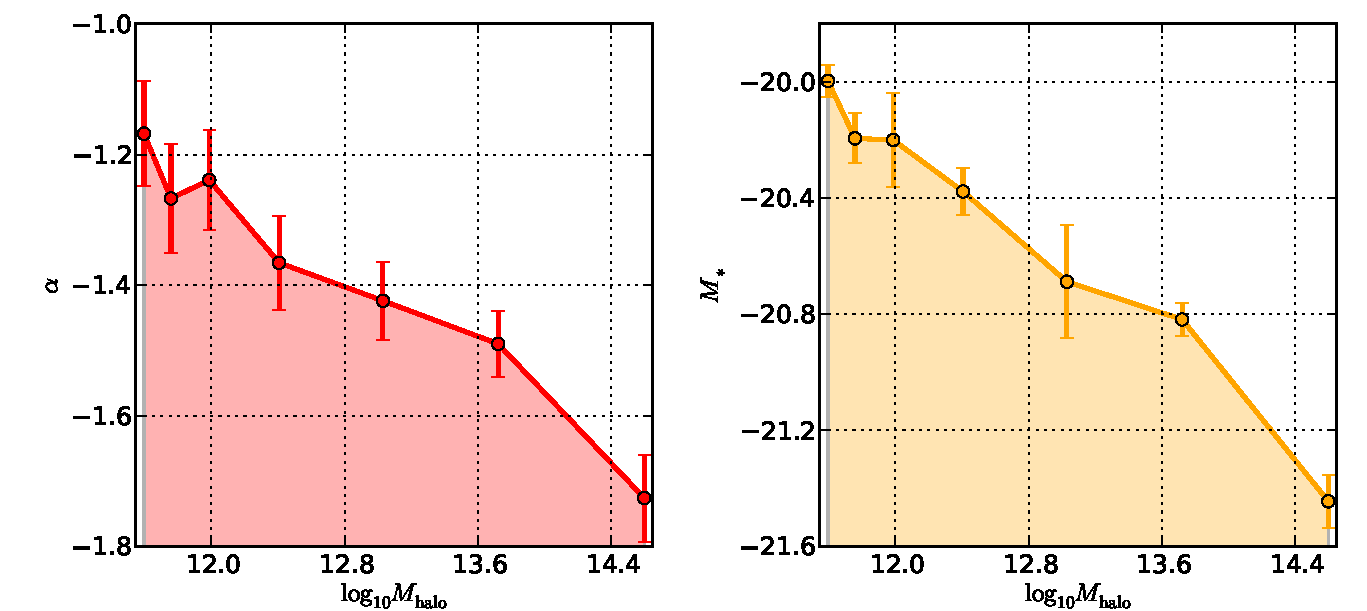
\includegraphics[width=0.8\linewidth]{evolSchechterLinMockGalPop}
    \caption{Modulation of the parameters for a Schechter distribution with the
    halo mass in the mock catalogue constructed as described in the previous
figure. Parameters are recovered with a given uncertainties.}
\label{fig:paramschlinmock}
\end{figure}
